\ffigbox[\FBwidth]{%
\caption{\centering Graphe cubique utilisé pour construire \(G_1\)}\label{Fig:exam_blanc_ex_2_1}
}{
    \fbox{
        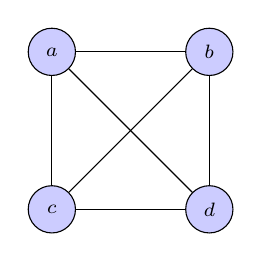
\begin{tikzpicture}[scale=1, main node/.style={circle, draw, fill=blue!20, inner sep=1pt, font=\scriptsize, minimum size=6mm}]
            % graphe complet de taille 4
            \node[main node] (a) at (0,2) {\(a\)};
            \node[main node] (b) at (2,2) {\(b\)};
            \node[main node] (c) at (0,0) {\(c\)};
            \node[main node] (d) at (2,0) {\(d\)};
            
            \draw (a) -- (b);
            \draw (a) -- (c);
            \draw (a) -- (d);

            \draw (b) -- (c);
            \draw (b) -- (d);

            \draw (c) -- (d);

        \end{tikzpicture}
    }
}